\chapter{Dostupná řešení}
\label{ch:existing}
V následující kapitole je představeno 7 komerčně nabízených softwarových balíků, které souvisí se zajištěním chodu kempu a jsou alespoň částečně přizpůsobeny české legislativě.
Následně budou představeny 2 závěrečné vysokoškolské práce, které vznikly na Vysokém učení v Brně.
Poslední část je věnována zhodnocení popsaných řešení a zdůvodnění tvorby této práce.

\section{Komerční řešení}
Při analýze současného trhu s informačními systémy pro ubytovací zařízení je patrná značná diverzifikace produktů, které se snaží pokrýt široké spektrum potřeb od malých penzionů až po rozsáhlé hotelové řetězce.
Tato kapitola se zaměřuje na zhodnocení dostupných komerčních platforem a především schopnost adaptace na specifické provozní podmínky turistických kempů.
Cílem rešerše je identifikovat silné stránky etablovaných systémů, ale také odhalit jejich limitace, které v kontextu sezónního provozu často spočívají v přílišné komplexnosti, vysokých provozních nákladech nebo v absenci úzce specializovaných funkcí.

\subsection{Better Hotel}
Systém Better Hotel\footnote{Dostupné z: \url{https://better-hotel.com/cs/}} působí na první pohled jako funkčně bohaté cloudové PMS\footnote{Property Management System} SaaS\footnote{Software as a~Service} řešení, nicméně zkouška praktického nasazení v~prostředí kempů by odhalila řadu zásadních nedostatků.
Při analýze reálných nasazení (např. Kemp Džbán\footnote{Dostupné z: \url{https://www.campdzban.eu/cs/ubytovani/}.}, Kemp Litovel\footnote{Dostupné z: \url{https://www.in-life.cz/rezervace-chatky}.}) a~demo verze se ukazuje, že veřejné rezervační rozhraní je částečně nefunkční nebo spíše často nekonzistentní a~pro uživatele zmatečné.
V~některých případech nefungují odkazy vůbec, jinde je rezervační proces sice dostupný, avšak omezený pouze na jednotlivé chaty bez možnosti agregovaného pohledu na obsazenost skupin objektů.
V~kontextu kempového provozu to znamená, že zákazník (nebo obsluha) musí ručně proklikávat desítky objektů, aby zjistil dostupnost, což je z~hlediska použitelnosti i~efektivity provozu krajně nevhodné a~neodpovídá reálným potřebám tohoto typu zařízení.

Významným problémem systému je uživatelské rozhraní, které působí nepřehledně a~mís-ty nedotaženě.
Při práci v~administraci dochází k~častému nesmyslnému překryvu UI prvků, které nevyvolávají žádnou akci, některé části rozhraní jsou ořezané tak, že není zobrazen celý obsah, a~práce s~delšími seznamy vyžaduje nadměrné scrollování, které se zasekává, viz obrázek \ref{fig:better-hotel}.
Systém se silně opírá o~modální dialogová okna, která jsou někdy používána i~pro potvrzovací akce, jindy bez zjevné logiky, což zvyšuje kognitivní zátěž uživatele.
Problematické jsou rovněž texty a~hlášení v~UI\,--\,například po otevření přihlašovacího odkazu se zobrazí informace o~odhlášení, což je z~pohledu UX matoucí.
Tyto nedostatky vytvářejí dojem, že frontend není dostatečně testován z~hlediska reálných uživatelských scénářů, zejména v~prostředí s~vysokou fluktuací hostů a~personálu.

Z~provozního hlediska není Better Hotel vhodný pro rychlé odbavování hostů typické pro kempy, ale spíše pro klasický hotelový provoz.
Celý systém implicitně předpokládá, že host má rezervaci předem, vše je zaplaceno online a~případně proběhne i~online check-in.
Tento model neodpovídá realitě kempů, kde jsou běžné nárazové příjezdy, krátkodobé pobyty a~potřeba velmi rychlého odbavení na recepci.
Administrace navíc obsahuje koncepčně sporné prvky, jako je správa \uv{ubytovacího poplatku}, který není v~praxi kempů standardizovaný a~působí spíše jako účetní konstrukt poskytovatele než reálný provozně-právní požadavek.
Přestože systém jako celek působí funkčně bohatě, celkový dojem je, že není dostatečně odladěn pro specifické potřeby kempového provozu; zejména frontend vyvolává pochybnosti o~kvalitě implementace, ačkoliv stav backendu nelze z~pohledu uživatele jednoznačně posoudit.

\begin{figure}
    \centering
    
\includegraphics[width=0.75\linewidth]{better-hotel.png}
    \caption{Ukázka rezervační plachty v~systému Better hotel.}
    \label{fig:better-hotel}
\end{figure}

\subsection{Bookio}
Bookio\footnote{Dostupné z: \url{https://www.bookio.com/cs}} představuje rozsáhlý cloudový rezervační systém zaměřený primárně na trh střední a~východní Evropy, což je patrné zejména z~kvalitní české lokalizace a~deklarované podpory evropské legislativy (GDPR, VOP).
Systém je vyvíjen slovenskou společností a~je koncipován jako univerzální řešení pro velmi široké spektrum odvětví – od wellness a~zdravotnictví přes gastronomii až po ubytovací zařízení.
Právě tato silná sektorová diverzifikace však naznačuje, že Bookio není primárně specializovaným PMS systémem, ale spíše obecnou rezervační platformou, která se snaží pokrýt co největší množství use-case scénářů.
V~oblasti ubytování systém formálně podporuje hotely, penziony, chaty a~apartmány, nicméně již z~prezentace je patrné, že se jedná spíše o~adaptaci obecného rezervačního modelu než o~řešení navržené přímo pro specifické potřeby tohoto segmentu.

Z~hlediska ověřitelnosti funkcí a~praktického nasazení je zásadním nedostatkem systému Bookio absence veřejně dostupné demo verze a~nedostatek referencí.
Přestože jsou funkce systému podrobně popsány na oficiálních stránkách, není možné si je nezávisle vyzkoušet ani dohledat konkrétní ubytovací zařízení, která by systém aktivně používala.
To významně komplikuje objektivní hodnocení kvality implementace, použitelnosti rozhraní i~reálné přidané hodnoty pro provozovatele.
V~kontextu diplomové práce a~analýzy existujících řešení je tento aspekt problematický, neboť znemožňuje porovnání deklarovaných vlastností s~reálným provozem.
Absence referencí zároveň vyvolává otázky ohledně míry adopce systému v~praxi, zejména v~konkurenčním prostředí, kde jsou běžně dostupné PMS systémy s~doložitelným nasazením.

Z~architektonického a~koncepčního hlediska lze Bookio hodnotit jako robustní, avšak příliš obecné řešení, které se snaží pokrýt mnoho sektorů na úkor hloubky specializace.
Implementace evropských legislativních požadavků je bezesporu nezbytným minimem, nicméně systém zjevně neřeší specifika jednotlivých států ani provozní detaily typické pro konkrétní typy ubytovacích zařízení (např. kempy, sezónní provozy nebo rychlé odbavení hostů).
V~porovnání s~úzce zaměřenými PMS systémy tak Bookio působí spíše jako univerzální rezervační nástroj než jako plnohodnotný hotelový či kempový management systém.
Tento přístup může být výhodný pro menší provozy s~jednoduchými požadavky, avšak pro komplexnější scénáře představuje omezení, které by muselo být řešeno dalšími externími nástroji nebo úpravami.

\subsection{Dotykačka}
Dotykačka je primárně pokladní (POS) systém určený pro evidenci prodeje, skladů a~obsluhu provozu na místě, nikoliv plnohodnotný rezervační či ubytovací systém.
Nabízí varianty cílené na hotely a~kempy, avšak tyto moduly se soustředí zejména na evidenci tržeb, směn zaměstnanců, inventáře a~propojení s~účetnictvím, nikoliv na řízení rezervací nebo obsazenosti ubytovacích kapacit.
Z~tohoto pohledu Dotykačka řeší jinou část provozního řetězce než specializované PMS systémy.

Rezervační funkcionalita je v~systému dostupná pouze nepřímo a~velmi omezeně.
Teoreticky by bylo možné využít obecný rezervační modul (např. rezervace stolů), nicméně jeho přizpůsobení pro ubytování by znamenalo výraznou administrativní zátěž a~obcházení původního účelu systému.
Chybí zde nativní podpora práce s~pobyty, více nocemi, typy ubytování, obsazeností nebo cenovými modely typickými pro kempy a~ubytovací zařízení.

Dotykačka tak může vhodně doplňovat ubytovací systém jako POS řešení pro místní prodej, nikoliv jej nahrazovat.
Z~hlediska této práce proto představuje spíše podpůrný nástroj než relevantní alternativu k~navrhovanému systému a~její využití v~oblasti rezervací je omezené a~koncepčně nevhodné.

\subsection{DrIngs RECEPCE}
Systém RECEPCE od společnosti Drings\footnote{Dostupné z: \url{https://www.drings.cz/software/recepce/}} představuje specializované softwarové řešení zaměřené primárně na provoz recepcí autokempů a~obdobných ubytovacích zařízení, které se v~současné době v~Kempu Olšovec používá.
Na rozdíl od obecně pojatých cloudových PMS systémů je jeho koncepce výrazně orientována na praktický provoz v~terénu, kde je klíčová rychlost odbavení hostů, práce s~fyzickou recepcí a~schopnost fungovat i~při omezené dostupnosti internetu.
Základní varianta systému je desktopová aplikace provozovaná lokálně, přičemž se jedná o~2vrstevnou architekturu tlustého klienta (implementovaného v~jazyce C++ s~pomocí frameworku QT) a~databáze (MS SQL server).
Její UI je možné zhlédnout na obrázcích \ref{fig:recepce-01} a~\ref{fig:recepce-02}.

Funkčně systém pokrývá běžné činnosti recepce, jako je evidence pobytů, správa obsazenosti, vystavování dokladů, práce s~platbami a~generování povinných výstupů.
Významnou výhodou je orientace na české legislativní prostředí.
Systém rovněž podporuje napojení na externí čtečky dokladů, což zvyšuje jeho využitelnost při fyzickém odbavování hostů přímo na recepci.

Součástí systému je také modul objednávek ubytování, který umožňoval správu rezervací.
Tento modul byl v~praxi určitý čas používán, avšak provozní zkušenosti ukázaly řadu problémů, zejména z~hlediska spolehlivosti a~použitelnosti v~reálném provozu.
Z~těchto důvodů bylo od jeho aktivního používání v~Kempu Olšovec upuštěno a~přešlo se na používání aplikace Excel.

Webová nadstavba RECEPCE-ONLINE rozšiřuje desktopovou aplikaci o~možnost online rezervací prostřednictvím webového rozhraní.
Rezervace vytvořené zákazníkem jsou přímo zapisovány do centrální databáze systému, což eliminuje nutnost ruční synchronizace mezi webem a~recepcí.
Tento přístup představuje významný posun oproti čistě lokálním řešením a~umožňuje alespoň základní formu digitalizace rezervací.
Zároveň však rezervační modul zůstává relativně jednoduchý a~jeho využívání nedává smysl vzhledem k~faktu, že modul Objednávek není využíván.

Z~celkového pohledu lze systém Drings RECEPCE hodnotit jako praktické a~provozně ověřené řešení pro tradiční recepční práci v~kempech, které dobře pokrývá administrativní a~legislativní požadavky českého prostředí.
Jeho slabší stránkou je technologická koncepce vycházející ze starší lokální desktopové aplikace, která je ale udržovaná, omezený rozsah online funkcí a~chování v~okrajových situacích.

\begin{figure}
    \centering
    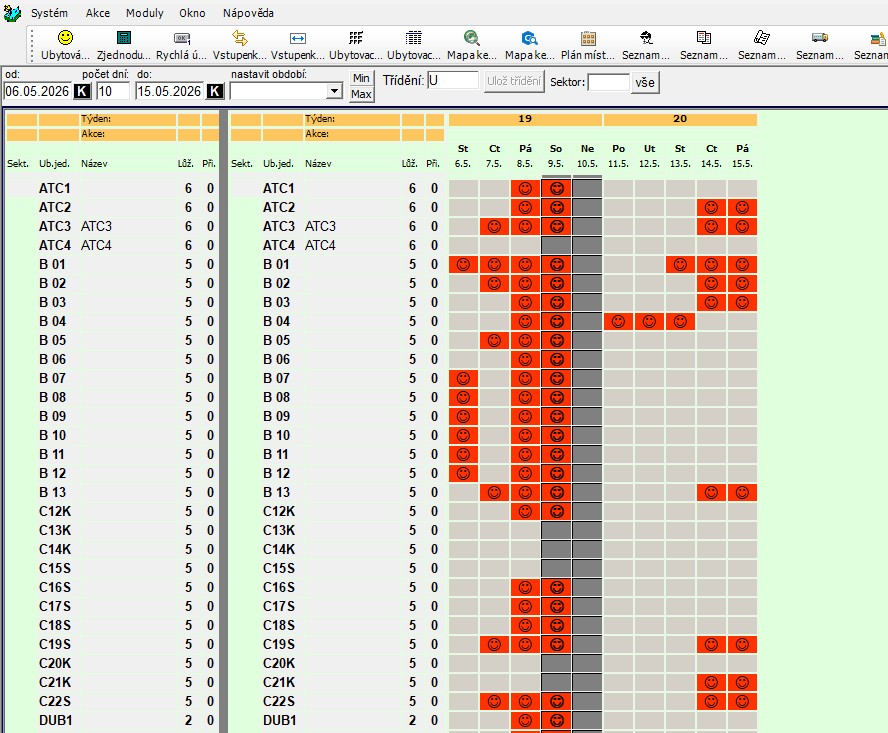
\includegraphics[width=0.75\linewidth]{figures/recepce-01.jpg}
    \caption{Plachta rezervací v~softwaru Recepce\protect\footnotemark.}
    \label{fig:recepce-01}
\end{figure}
\footnotetext{Dostupné z: \url{https://www.drings.cz/wp-content/uploads/2024/01/09_UbytovaciPlan_408x0.jpg} [cit. 10. prosince 2025].}

\begin{figure}
    \centering
    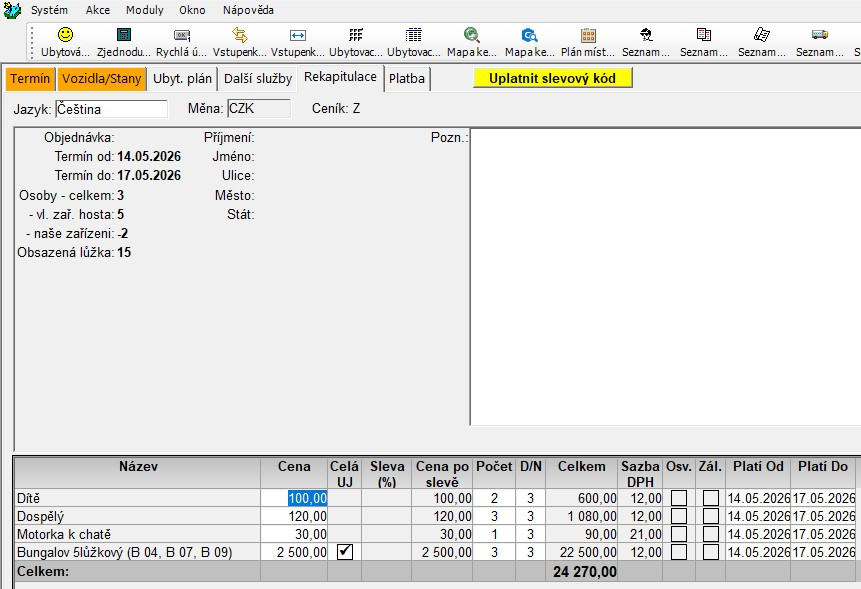
\includegraphics[width=0.75\linewidth]{figures/recepce-02.jpg}
    \caption{Kontrolní rekapitulace účtovaných služeb v~softwaru Recepce\protect\footnotemark.}
    \label{fig:recepce-02}
\end{figure}
\footnotetext{Dostupné z: \url{https://www.drings.cz/wp-content/uploads/2024/01/01_UbytUctRekapitulace_408x0.jpg} [cit. 10. prosince 2025].}

\subsection{Previo}
Systém Previo\footnote{Dostupné z: \url{https://www.previo.cz/}} představuje jeden z~nejpokročilejších a~velice rozšířených ubytovacích systémů na českém trhu.
Již na první pohled je patrné, že se jedná o~aktivně vyvíjenou platformu s~velmi kvalitní a~detailní dokumentací, která pokrývá jak technické aspekty systému, tak i~provozní scénáře z~pohledu recepce a~managementu, viz obrázek \ref{fig:previo}.
Dokumentace je přehledná, konzistentní a~naznačuje vysokou míru profesionality i~dlouhodobě řízeného vývoje.

Z~funkčního hlediska se jedná o~velmi komplexní a~technicky vyspělý systém, který nabízí propracovanou správu rezervací, práci s~cenami, reporty, channel management i~napojení na externí služby.
Systém je zpracován jako cloudové Saas řešení s~centrální správou dat a~pravidelnými aktualizacemi.
Tento přístup je vhodný zejména pro hotely, penziony a~zařízení s~vysokým podílem předem vytvořených rezervací.
Přes vysokou míru technologické vyspělosti však systém postrádá podporu některých lokálně specifických nástrojů, zejména integraci eDokladů, což je v~kontextu českého prostředí a~povinností ubytovatelů významné omezení.

Z~pohledu provozu kempů a~obdobných zařízení se však ukazuje, že Previo není optimalizováno pro scénáře s~vysokým náporovým provozem na recepci a~s~velkým podílem hostů bez předchozí rezervace.
Systém, který se sám prezentuje jako hotelový, implicitně předpokládá, že většina pobytů vzniká na základě rezervací vytvořených předem, a~workflow recepce je tomu přizpůsobeno.
V~prostředí kempů, kde hosté často přijíždějí bez rezervace a~je nutné je rychle odbavit, tento přístup zpomaluje práci a~zvyšuje administrativní zátěž personálu.
Chybí zde rovněž specializované komponenty pro evidence vozidel, stanů a~dalších dočasných ubytovacích jednotek, které jsou pro kempový provoz zásadní a~nelze je efektivně modelovat pomocí standardních hotelových pokojů.

Celkově lze Previo hodnotit jako vysoce kvalitní, technicky vyspělé a~dobře zdokumentované řešení, které je vhodné především pro klasická ubytovací zařízení s~organizovaným rezervačním procesem.
Jeho slabinou, v~kontextu této práce, je však nedostatečné přizpůsobení specifickým potřebám kempů a~sezónních provozů, kde dominují spontánní příjezdy, rychlé odbavení a~práce s~nestandardními ubytovacími jednotkami.
V~kontextu této práce tak Previo představuje silné referenční řešení z~pohledu implementovaných funkcionalit, nikoliv však systém optimálně navržený pro cílový typ zařízení, na který se práce zaměřuje.

\begin{figure}
    \centering
    
\includegraphics[width=0.75\linewidth]{previo.png}
    \caption{Ukázka UI systému Previo na různých zařízení\protect\footnotemark.}
    \label{fig:previo}
\end{figure}
\footnotetext{Dostupné z: \url{https://www.previo.cz/wp-content/uploads/2024/03/recepcni-system.webp} [cit. 10. prosince 2025].}

\subsection{Rezeo}
Systém Rezeo\footnote{Dostupné z: \url{https://rezeo.cz/sluzby}} je prezentován jako jednoduchý online rezervační nástroj určený především pro samostatné objekty, zejména chaty a~chalupy.
Tomu odpovídá i~jeho celková koncepce, která se soustředí na minimální administrativní zátěž a~automatizaci základního rezervačního procesu.
Rezeo je typickým příkladem řešení navrženého pro malé provozy s~nízkou frekvencí hostů, kde není potřeba komplexní recepční systém ani pokročilé řízení provozu.

Z~funkčního hlediska systém implicitně předpokládá platbu předem jako standardní součást rezervačního procesu.
Tento přístup může být vhodný pro objekty pronajímané na celé pobyty s~jasně definovanými termíny, avšak vylučuje scénáře, kde je běžné platit až na místě nebo kde dochází k~častým změnám a~prodlužování pobytů.
Rezeo rovněž neřeší žádné zákonné povinnosti ubytovatelů.
Z~tohoto důvodu systém nelze považovat za plnohodnotné řešení pro provoz ubytovacího zařízení v~českém legislativním prostředí.

Zásadním omezením systému je také absence technické a~uživatelské dokumentace.
K~dispozici jsou pouze marketingově laděné FAQ, které vysvětlují základní principy fungování, nikoliv detailní popis chování systému, integračních možností nebo chybových stavů.
To výrazně komplikuje jak hlubší analýzu systému, tak jeho případné rozšíření nebo integraci s~dalšími nástroji.
Rezervační formulář určený k~vložení na webové stránky je navíc poměrně jednoduchý a~funkčně omezený, bez pokročilejší práce s~dostupností, variantami ubytování či doplňkovými službami.

Z~pohledu provozu kempů nebo zařízení s~vysokým náporovým odbavováním hostů není Rezeo vhodným řešením.
Systém není optimalizován pro rychlé odbavování na místě, nepodporuje práci bez rezervace a~nepokrývá evidenci typickou pro sezónní a~plošné provozy.
Celkově tak Rezeo představuje úzce zaměřený rezervační nástroj pro malé, samostatné objekty, nikoliv univerzální nebo rozšiřitelné řešení, které by bylo schopné obsloužit složitější provozní scénáře.

\subsection{WebPortýr}
Systém Webportýr je koncipován jako čistě rezervační nástroj, jehož hlavním cílem je zprostředkování online rezervací ubytování prostřednictvím webového rozhraní.
Funkčně se soustředí především na prezentaci dostupnosti, příjem rezervací a~základní komunikaci se zákazníkem.
Z~tohoto pohledu se nejedná o~plnohodnotný PMS či recepční systém, ale spíše o~doplňkovou službu určenou k~získávání rezervací.

Zásadním omezením systému je skutečnost, že neřeší provozní ani legislativní aspekty ubytování.
Chybí zde podpora povinností vyplývajících z~české legislativy, jako je evidence ubytovaných osob, práce s~poplatky z~pobytu, vazba na cizineckou policii nebo další administrativní úkony, které jsou pro provozovatele ubytovacích zařízení nezbytné.
Systém tedy nepokrývá celý životní cyklus pobytu hosta, ale pouze jeho úvodní rezervační fázi.

Z~pohledu této práce lze Webportýr hodnotit jako velmi úzce specializované řešení, které může sloužit jako rezervační nadstavba k~jinému informačnímu systému, nikoliv však jako samostatný nástroj pro řízení provozu ubytovacího zařízení.
Absence legislativních funkcí a~provozních evidencí jej činí nevhodným jako komplexní řešení, zejména v~českém prostředí, kde jsou administrativní povinnosti ubytovatelů výrazné a~nelze je opominout.
\section{Vysokoškolské závěrečné práce}
Prohledáním portálu Vysokoškolských kvalifikačních prací\footnote{Dostupné z: \url{https://theses.cz/}} v České republice byly objeveny 2 relevantní závěrečné práce zaměřující se na problematiku informačního systému pro ubytování.
Obě dvě práce byly vypracovány na Vysokém učení technickém v Brně.

První práci s názvem \uv{Informační systém ubytovacích služeb} vypracoval Ondřej Zelinka pod vedením dr. Zbyňka Křivky \cite{bp-zelinka}.
Tato práce sepsaná v akademickém roce 2022/2023 se zaměřuje na návrh a implementaci webového informačního systému pro  Salesiánský klub mládeže z.s. Dům Ignáce Stuchlého, pro nějž je typické ubytování nikoliv jednotlivců, nýbrž skupin.
Návrh a implementace se tedy zabývá ubytováním a objednávkou stravy pro tyto skupiny, a to nejen z pohledu databáze a implementace, ale i uživatelského rozhraní.
Realizační výstup práce je dle oponentského posudku použitelný a kvalitně vypracovaný.
Přesto je práce hodnocena stupněm C především z důvodu nedodržení formálních náležitostí technické zprávy.
Tato práce se zaměřuje pouze na jednu část požadavků popsaných v sekci \ref{sec:pozadavky}\,--\,skupinové rezervace ubytování a objednávky stravy.
Ačkoliv ostatní požadavky nejsou žádným způsobem řešeny, určité pasáže mohou být inspirativní pro vypracování této práce.

Druhou nalezenou práci vytvořil Jan Škrabal pod vedením dr. Jiřího Hynka s názvem \uv{Informační systém pro ubytovací zařízení} \cite{bp-skrabal}.
Student spolupracoval s Masarykovou střední školou Letovice, která řešila problematiku přístupu ubytovaných hostů do ubytování při jejich pobytu.
Řešení tohoto problému vyřešil pomocí ovládání mobilní aplikací s využitím technologie Bluetooth a mikrokontroléru ESP32 a elektronického zámku.
Ačkoliv se podobnému problému, otvírání závor, věnuji též, jedná se o napojení na externí systém, nikoliv samotné ovládání přístupového systému hardwarově.
Oproti práci od pana Zelinky se mírně věnuje legislativním náležitostem\,--\,konkrétně statistickým reportům na Český statistický úřad.
Ostatní nutnosti opomíjí, ačkoliv se přímo nabízejí.

\subsection{Vyhodnocení analýzy dostupných řešení}
Analýza ukázala, že současné systémy dostupné na trhu pokrývají rezervační a recepční procesy pouze částečně a často jsou zaměřeny na úzce vymezené scénáře.
Většina nástrojů se orientuje buď na správu rezervací, nebo na recepční provoz, avšak jen výjimečně zajišťují plnou podporu české legislativy, včetně evidence ubytovaných osob, hlášení cizinců a práce s poplatky z pobytu.
Některá řešení postrádají dokumentaci, jiná jsou koncipována pro chaty či malé objekty, případně se jedná pouze o rezervační widgety.
Pro sezónní a nárazově zatížené provozy, jako jsou právě turistické kempy, se navíc ukazuje jako nedostatečná optimalizace na rychlé odbavení hostů a efektivní práci recepce.

Navrhovaný systém reaguje na zjištěné nedostatky prostřednictvím čtyř zásadních konceptů: otevřenosti, legislativní úplnosti, provozní efektivity a kompletního fungování v digitálním prostředí.
Open-source charakter řešení umožňuje transparentní kontrolu kódu, snadnou rozšiřitelnost a možnost komunitního přispívání, což u komerčních systémů převážně chybí.
Žádný podobný software s otevřeným zdrojovým kódem v České republice není a díky přeregulování českého a evropského právního prostředí pravděpodobně ani nebudou existovat.
Důsledná implementace české legislativy eliminuje nutnost manuálních obcházek a minimalizuje riziko chyb například při evidenci hostů.
Optimalizace systémů na rychlé odbavování není navržena tak, aby systém podporoval plynulý provoz i v situacích s vysokou koncentrací příchozích hostů, což pro kempy představuje klíčovou výhodu i nutnost.
